\section{Property Reification}
\label{sec:Property}
%%%%%%%%%%%%%%%%%%%%%%%%%%%%%%%%%%%%%%%%%%%%%%%%%%%%%%%%
\begin{figure}[h!]
\begin{center}
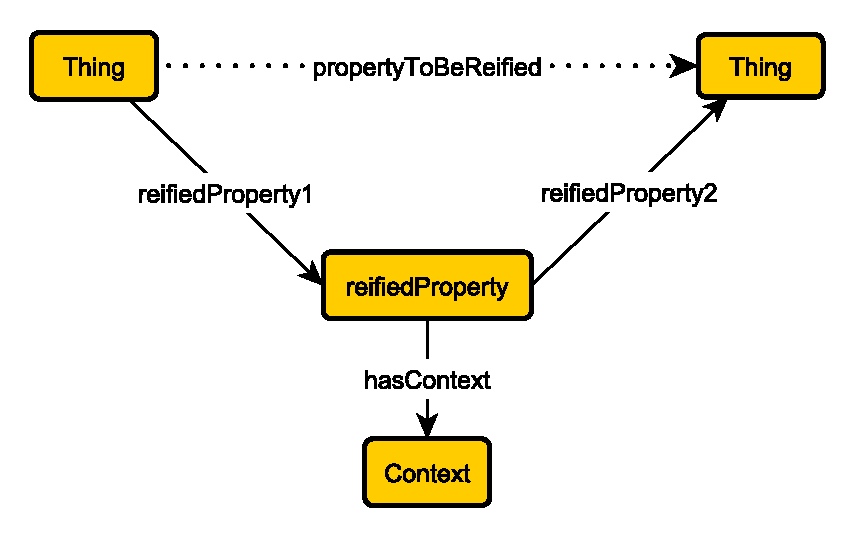
\includegraphics[width=.7\textwidth]{figures/reification}
\end{center}
\caption{Schema Diagram for Property Reification. The visual notation is explained in Chapter \ref{chap:prelims}. Additioanlly, we use the dotted line with solid arrow to indicate which property is being reified. This relation has no bearing on the below axioms.}
\label{fig:Property}
\end{figure}
\subsection{Summary}
\label{sum:Property}
%%%%%%%%%%%%%%%%%%%%%%%%%%%%
The \textsf{AgentRole} pattern is essentially a reification of association with something. That is, it's very unlikely that an Agent will be associated with something for all time. Thus, the association relation is not binary, perhaps $\textit{associated}(x,y,t)$, agent $x$ is associated with thing $y$ at time $t$. Thus, the reification. The association becomes a concept in its own right and has a temporal extent, allowing an \textsf{Agent} to be associated to a \textsf{Thing} (e.g. \textsf{Event}, Section \ref{sec:Event}) for some \textsf{TemporalExtent}.

%%%%%%%%%%%%%%%%%%%%%%%%%%%%%%%%%%%%%%%%%%%%%%%%%%%%%%%%
\subsection{Axiomatization}
\label{axs:Property}
%%%%%%%%%%%%%%%%%%%%%%%%%%%%
\begin{align}
\top &\sqsubseteq \forall\textsf{place.Holder} \\ 
\exists\textsf{place.Holder} &\sqsubseteq \top 
\end{align}

%%%%%%%%%%%%%%%%%%%%%%%%%%%%%%%%%%%%%%%%%%%%%%%%%%%%%%%%
\subsection{Explanations}
\label{exp:Property}
%%%%%%%%%%%%%%%%%%%%%%%%%%%%
\begin{enumerate}
\item temporary item
\end{enumerate}

%%%%%%%%%%%%%%%%%%%%%%%%%%%%%%%%%%%%%%%%%%%%%%%%%%%%%%%%
\subsection{Competency Question}
\label{cqs:Property}
%%%%%%%%%%%%%%%%%%%%%%%%%%%%
\begin{enumerate}[CQ1.]
\item temporary item
\end{enumerate}

\newpage
%%%%%%%%%%%%%%%%%%%%%%%%%%%%%%%%%%%%%%%%%%%%%%%%%%%%%%%%
% End Section
%%%%%%%%%%%%%%%%%%%%%%%%%%%%%%%%%%%%%%%%%%%%%%%%%%%%%%%%
%%%%%%%%%%%%%%%%%%%%%%%%%%%%%%%%%%%%%%%%%%%%%%%%%%%%%%%%